\chapter{Using Convolutional Neural Networks for $\nu_{\mu}$ CC event classification}\label{ch:cnn_results}
\section{Classification using CNN10000}

%-----------------------------Commenting out selection I original work------------------------------------------------------------------
\begin{comment}
\subsection{Classification of MC data using Selection I Original CC-Inclusive Filter}\label{sel1orig}

\begin{figure}[htp!]
\centering
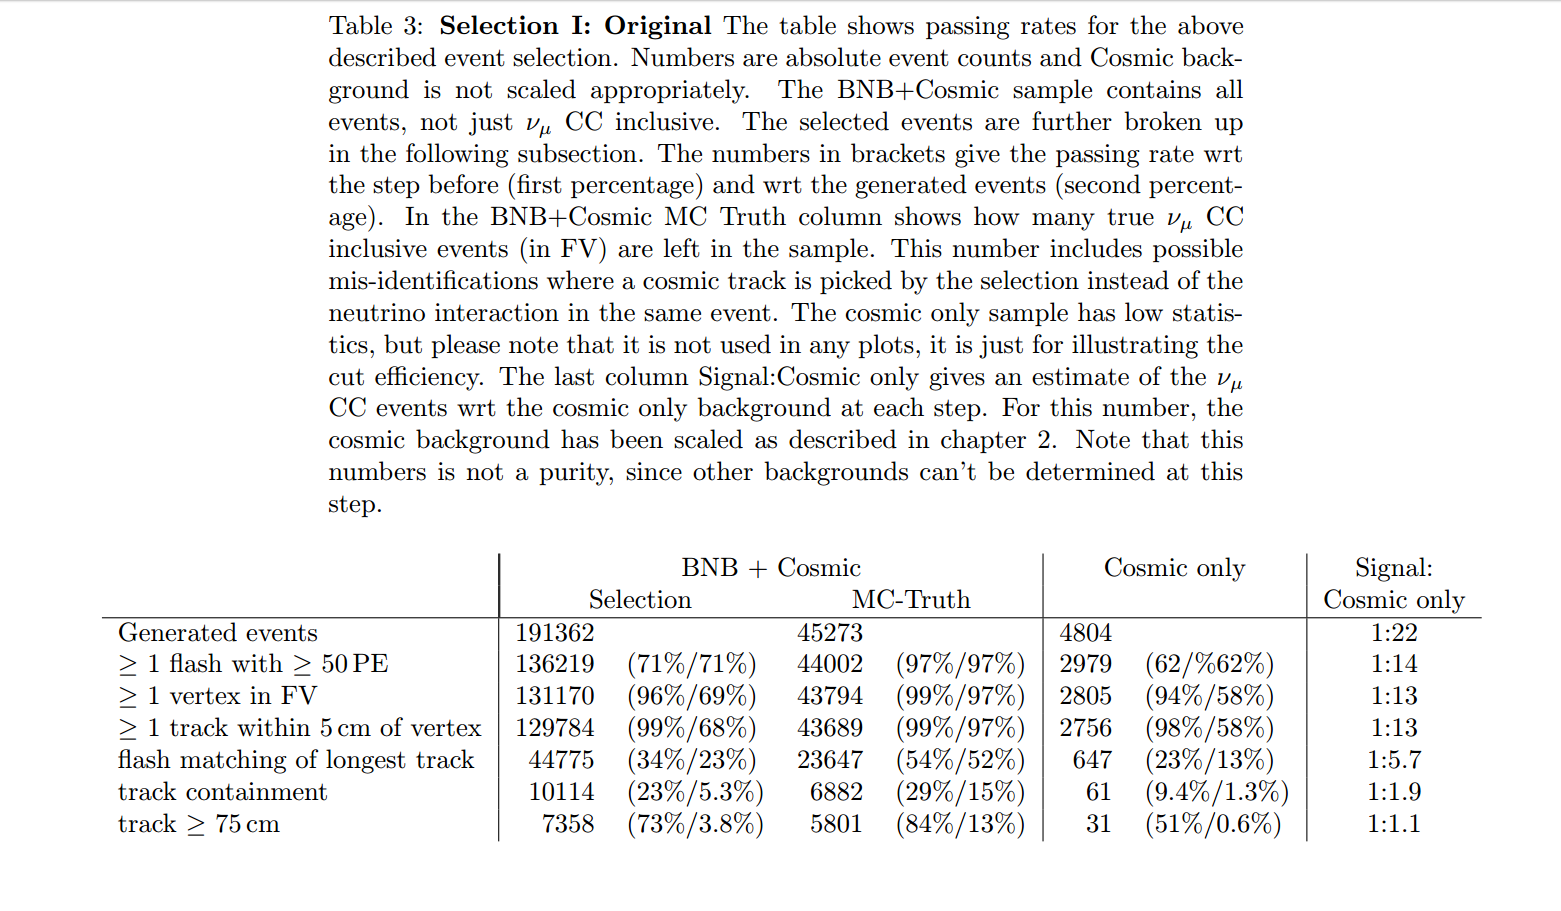
\includegraphics[width=.9\textwidth]{figs/sel1_cuts.png}
\caption{Snapshot of passing rates of Selection I from CC-Inclusive Filter} 
\label{fig:cuttable}
\end{figure}

\begin{figure}[htp!]
\centering
	\begin{subfigure}[b]{.45\textwidth}
	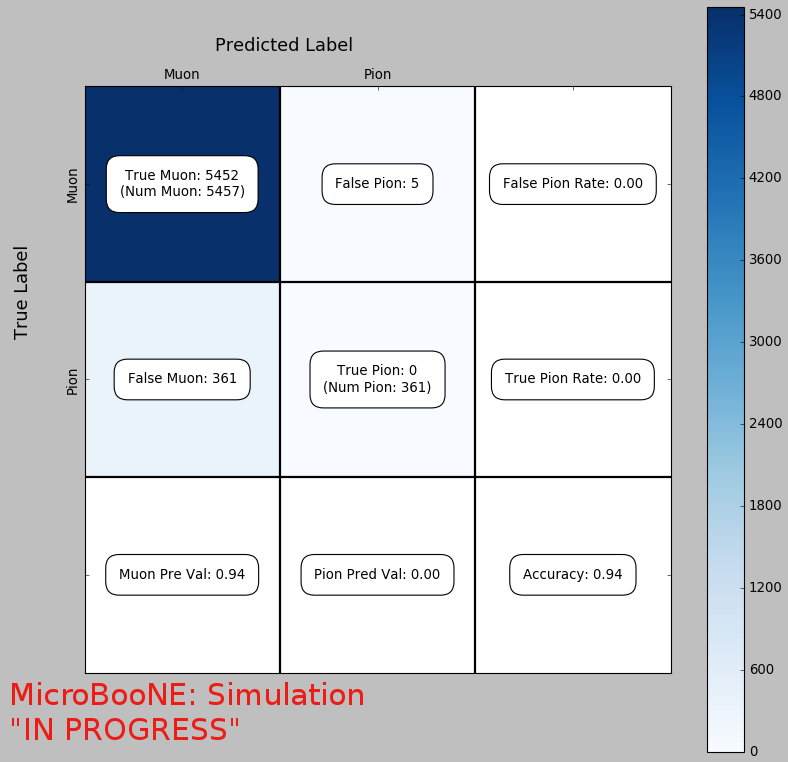
\includegraphics[width=3in,height=3in]{figs/confusion_0621_wrongnorm.png}
	\caption{Confusion Matrix showing Accuracy of CNN using data with wrong normilazion}
	\label{fig:confusion_wrongnorm}
	\end{subfigure}
	\quad
	\begin{subfigure}[b]{.45\textwidth}
	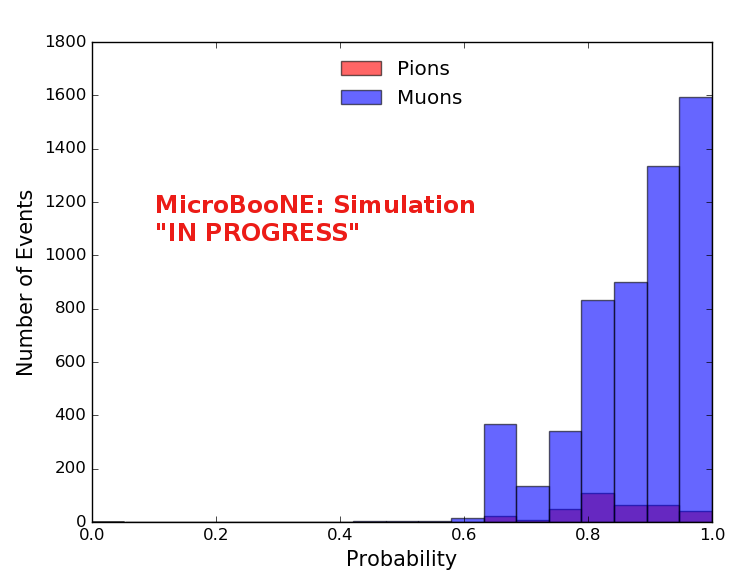
\includegraphics[width=3in,height=3in]{figs/prob_0706_wrongnorm_sel1.png}
	\caption{Probability plot showing $\mu/\pi$ separation of CNN using wrong normalization}
	\label{fig:prob_wrongnorm}
	\end{subfigure}
	\quad
	\begin{subfigure}[b]{.45\textwidth}
	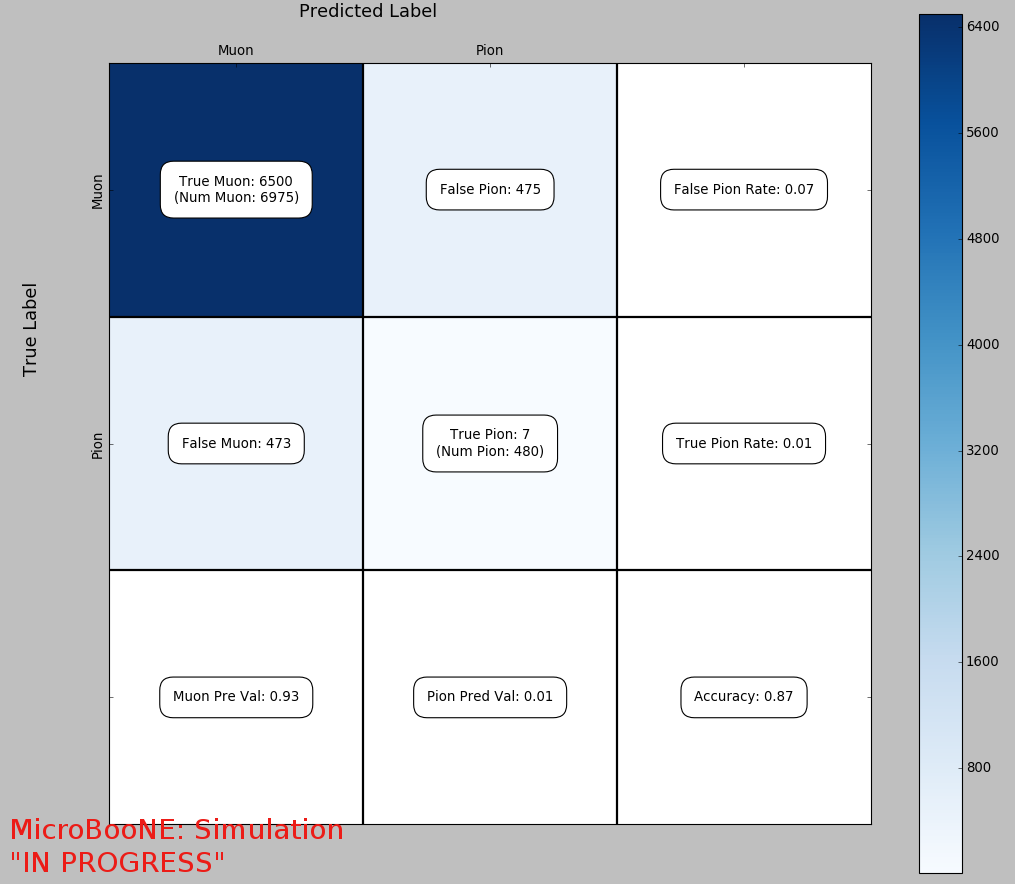
\includegraphics[width=3in,height=3in]{figs/confusion_rightnorm_0621.png}
	\caption{Confusion Matrix showing Accuracy of CNN using data with correct normilazion}
	\label{fig:confusion_rightnorm}
	\end{subfigure}
	\quad
	\begin{subfigure}[b]{.45\textwidth}
	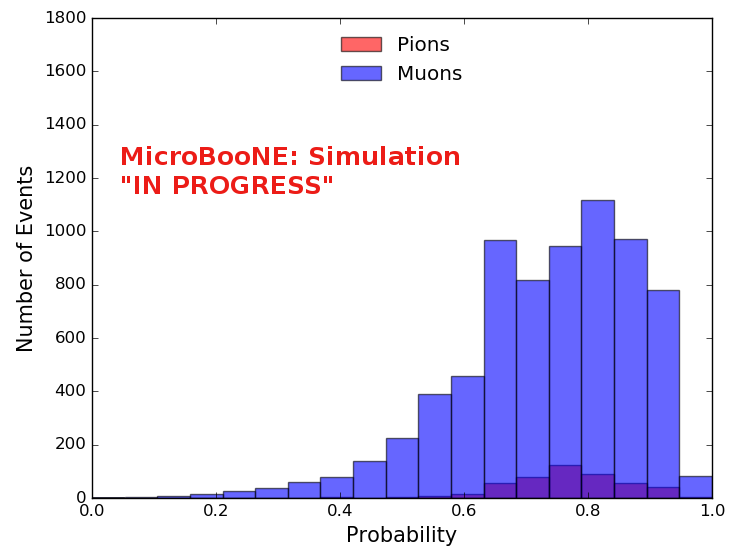
\includegraphics[width=3in,height=3in]{figs/prob_0706_rightnorm_sel1.png}
	\caption{Probability plot showing $\mu/\pi$ separation of CNN using correct normalization}
	\label{fig:prob_rightnorm}
	\end{subfigure}
	\quad
\caption{Results of CNN10000 classification of track candidate images output from cc-inclusive filter.}
\label{fig:CNN_ccnc}
\end{figure}

\begin{figure}[htp!]
\centering
	\begin{subfigure}[b]{.45\textwidth}
	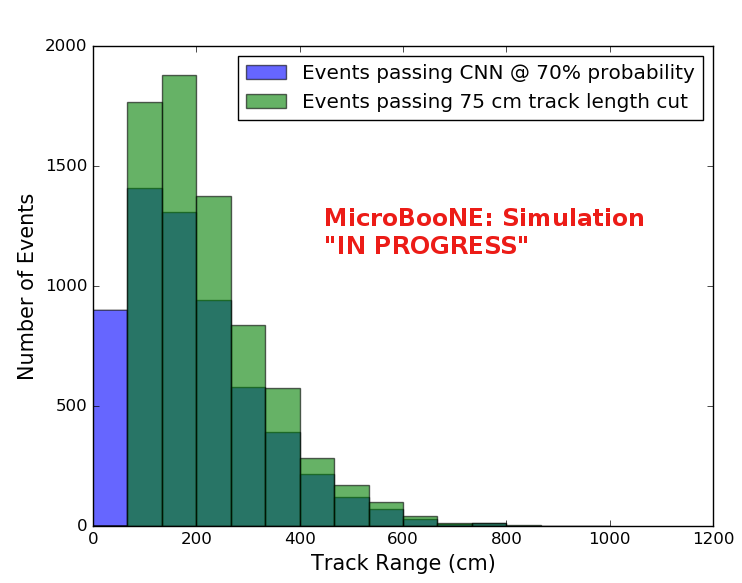
\includegraphics[width=3in,height=3in]{figs/sel1_trackrange_wrongnorm_acc70_0706.png}
	\caption{Track range distribution of events from Selection I Original passing CNN with 70\% accuracy using image data with wrong normilazion}
	\label{fig:track_wrongnorm}
	\end{subfigure}
	\quad
	\begin{subfigure}[b]{.45\textwidth}
	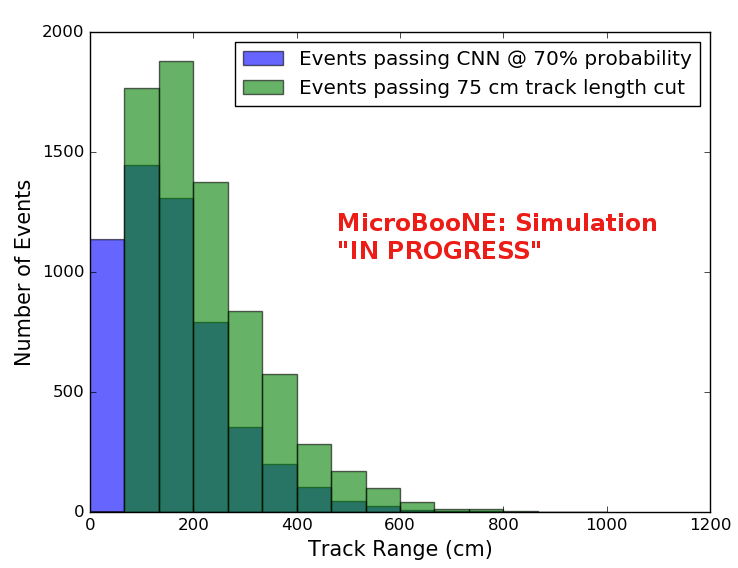
\includegraphics[width=3in,height=3in]{figs/sel1_trackrange_rightnorm_acc70_0706.png}
	\caption{Track range distribution of events from Selection I Original passing CNN with 70\% accuracy using image data with correct normilazion}
	\label{fig:track_rightnorm}
	\end{subfigure}
	\quad
	\begin{subfigure}[b]{.45\textwidth}
	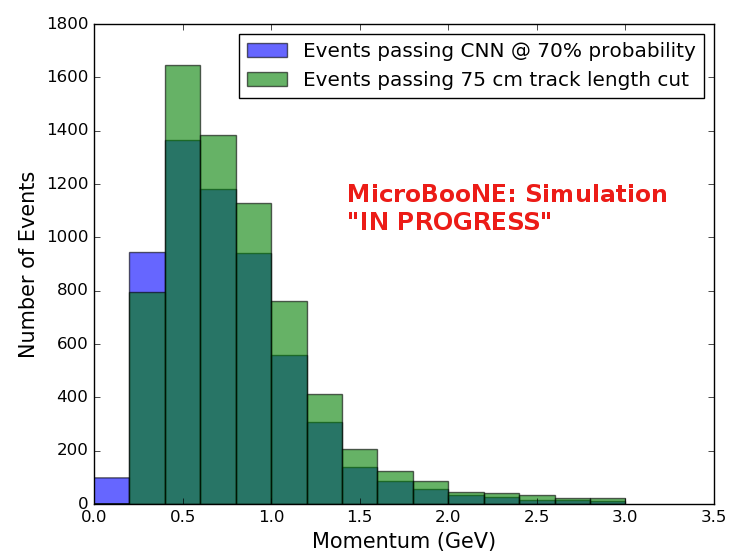
\includegraphics[width=3in,height=3in]{figs/sel1_parP_wrongnorm_acc70_0706.png}
	\caption{Momentum distribution of events from Selection I Original passing CNN with 70\% accuracy using image data with wrong normilazion}
	\label{fig:momentum_wrongnorm}
	\end{subfigure}
	\quad
	\begin{subfigure}[b]{.45\textwidth}
	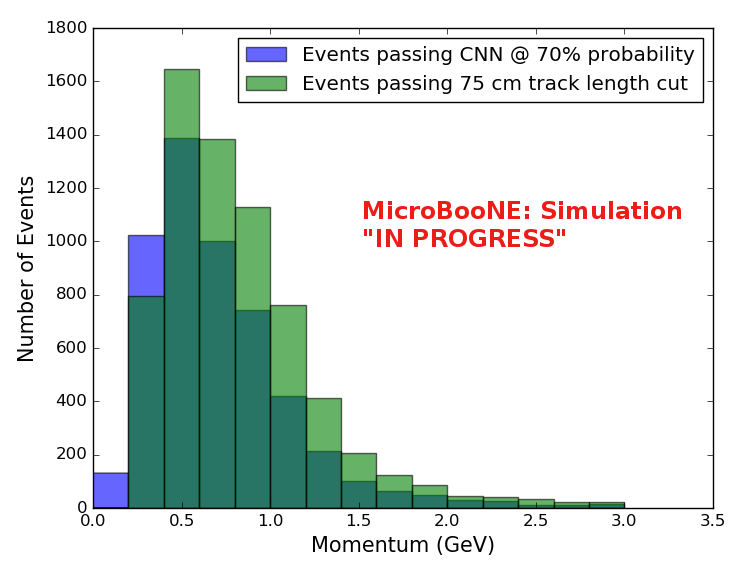
\includegraphics[width=3in,height=3in]{figs/sel1_parP_rightnorm_acc70_0706.png}
	\caption{Momentum distribution of events from Selection I Original passing CNN with 70\% accuracy using image data with correct normilazion}
	\label{fig:momentum_rightnorm}
	\end{subfigure}
	\quad
\caption{CNN10000 distributions of track candidate images output from Selection I Original cc-inclusive filter with different image data normalizations}
\label{fig:CNN_dist}
\end{figure}

The next step that was taken was to use CNN10000 to classify track candidate images that were identified by the selection I original cc-inclusive filter described in \cite{cc-inclusive}. Passing rates for each cut in cc-inclusive filter are show in figure \ref{fig:cuttable}. For the incorrect image making normalization dataset, out of 188,880 events, 7438 passed the cut right before 75 cm track length cut which is 3.9\% of total data. Discrepancies in passing rates are due to grid submission issues, however, this dataset is used to check if changes in image making normalization affects $\mu/\pi$ separation probability due to CNN10000 being trained with incorrectly image making normalized data. For the second dataset with correct image making normalization, out of 188,880 events, 9552 events passed the cut right before the 75 cm track length cut which is 5.1\% passing rate and is comparable to figure \ref{fig:cuttable}. In time cosmics were also run over for efficiency and purity calculations. Out of 14395 in time cosmic events, 175 passed the cut right before the 75 cm track length cut which is a passing rate of 1.2\% compared to 1.3\% shown in table \ref{table:mc} in section \ref{section:eventselection} . 

Figures \ref{fig:confusion_wrongnorm}, \ref{fig:prob_wrongnorm}, \ref{fig:confusion_rightnorm} and \ref{fig:prob_rightnorm} show the accuracy and $\mu/\pi$ separation of both the correct and incorrect normalized images. The confusion matrices are only composed of $\mu/\pi$ data. Other particles passed the cc-inclusive filter before the 75 cm track length cut and were all mis-id'ed as muons. Since CNN10000 has not seen any particles other than muons and pions, it makes sense that those get mis-id'ed. Figures \ref{fig:prob_wrongnorm} and \ref{fig:prob_rightnorm} don't have $\mu/\pi$separation comparable to \ref{fig:prob_plot}, but \ref{fig:prob_wrongnorm} does skew to higher probabilities compared to \ref{fig:prob_rightnorm}. This is to be expected and further work on quantifying the performance of CNN10000 should use the incorrect image making normalization. It is also expected that the separation isn't as defined as the testing dataset for CNN10000. CNN10000 was trained and tested using single particle muons and pions and the track candidate dataset come from BNB+Cosmic events, not to mentions all track candidates have passed the cc-inclusive filter that tags "muon-like" tracks therefore the pions in this sample look much closer in muon topology than the network has seen. Also, these images were made from wire and time ticks associated to hits from the track candidate that passed the cc-inclusive filter. This is different from the training images where a bounding box was drawn over the total $\mu$ or $\pi$ interaction. Spurious energy deposition from a $\pi-Ar$ interaction is most likely not included in the BNB+Cosmic images due to the tracking algorithm. To remedy this, the neural network needs to see more "muon-like" pions and muons and pions from a neutrino interaction passing the cc-inclusive filter as well as a larger particle variety including protons, photons and electrons. Although $\mu/\pi$ separation is lacking, CNN10000 does an excellent job of classifying muons and using higher CNN probability can increase purity. Figures \ref{fig:track_wrongnorm}, \ref{fig:track_rightnorm}, \ref{fig:momentum_wrongnorm} and \ref{fig:momentum_rightnorm} show the track and momentum distributions for these two datasets. In both sets you have an increase in data in the bin below 75 cm and at bins below 0.5 GeV. These distributions were made with events classified with 70\% probability of being a muon regardless of true particle type. 
\end{comment}
%-----------------------------Commenting out selection I original work------------------------------------------------------------------

\subsection{Classification of MC data using Selection I CC-Inclusive Filter}

After training CNN10000, it was then used to classify track candidate images that were identified by the selection I cc-inclusive filter described in chapter \ref{ch:meas}. Passing rates for each cut in this filter are shown in table \ref{table:mc}. Out of 188,880 events, 19,112 passed the cut right before the 75 cm track length cut which is a 10.1\% passing rate and comparable to the 10\% passing rate shown in table \ref{table:mc}. In time cosmics were also run over, out of 14,606 in time cosmics events, 302 passed the cut right before the 75 cm track length cut which is a 2.1\% passing rate comparable to the 2.7\% passing rate in the cc-inclusive tech-note. Figures \ref{fig:confusion_sel1mod} and \ref{fig:prob_sel1mod} show the accuracy and $\mu/\pi$ separation. Both plots are only composed of muons and pions due to the focus on $\mu/\pi$ separation and the fact that CNN10000 was only trained on muons and pions, however, for reference, all other particles that did pass selection I were mis-id'ed as muons. Muons are being identified at a very high rate, while pions are all being mis-id'ed as muons. This is due in part because the pion track candidate that does pass the cc-inclusive filter right before the 75 cm track length cut has already been identified as a muon candidate, hence, at a higher muon probability. Another reason for the pion mis'id can be attributed to the training/classifying dataset difference. For training, the pion images include the whole pion interaction in argon, including any decays or nucleon scattering. The image created from a BNB+Cosmic event used for classification only includes the track candidate that passed the cc-inclusive filter.
Figure \ref{fig:sel1mod_track} shows the track range distributions of all events from selection I being classified by the CNN as a muon with a probability of 70\% regardless of true particle type. We get entries for the CNN curve in the lowest bin and none for the 75 cm curve. To see how many true CC events were identified by CNN10000 breaking down figure \ref{fig:sel1mod_track} by event type was necessary. Figures \ref{fig:sel1mod_stackedcnn} and \ref{fig:sel1mod_stackedoriginal} show track range distributions separated by signal and various backgrounds. Particle type was not taken into consideration in these plots so true CC event images can be any track candidate particle passing selection I cut right before track length cut including pions and protons. 

To gain an even deeper understanding on how CNN10000 is performing, plotting these distributions with only muons and pions was done due to the fact that CNN10000 was trained with only those particles for $\mu/\pi$ separation. Figures \ref{fig:sel1mod_mupi_70stackedcnn}-\ref{fig:sel1mod_mupi_90stackedcnn} show the stacked histograms of signal and background of the track range distributions with varying CNN probabilities starting from 70\% and ending at 90\% probability. With higher probabilities we get a purer sample in the lower bin but we end up losing events as well. Momentum distributions for all signal/background events are shown in figure \ref{fig:sel1mod_parP}.    

\begin{figure}[htp!]
\centering
	\begin{subfigure}[b]{.45\textwidth}
	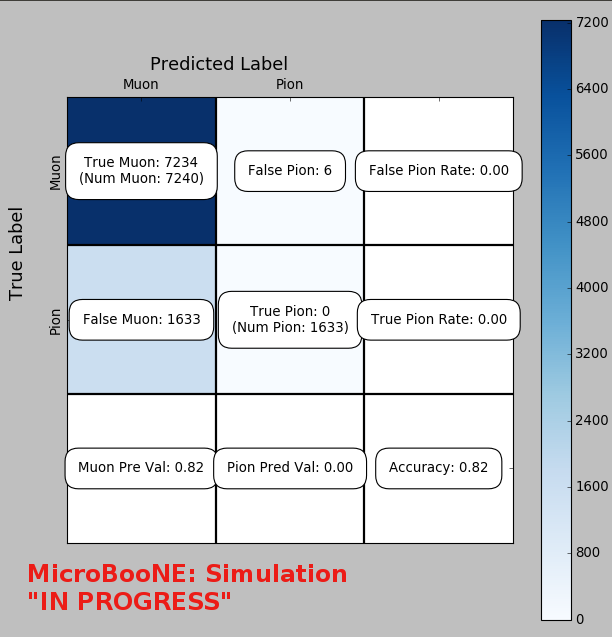
\includegraphics[width=3in,height=3in]{figs/sel1mod_confusion_wrongnorm.png}
	\caption{Confusion Matrix for CNN10000 classified events from selection I}
	\label{fig:confusion_sel1mod}
	\end{subfigure}
	\quad
	\begin{subfigure}[b]{.45\textwidth}
	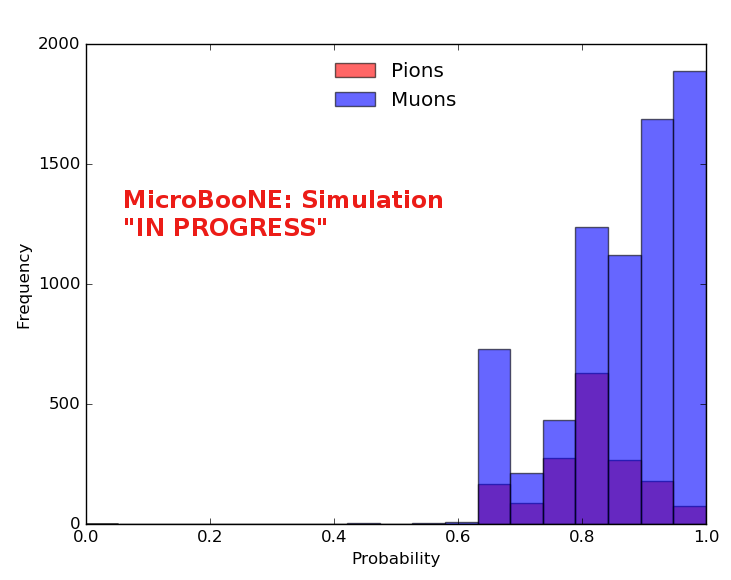
\includegraphics[width=3in,height=3in]{figs/probplot_wrongnorm_selImod.png}
	\caption{Probability plot for CNN10000 classified events from selection I}  
	\label{fig:prob_sel1mod}
	\end{subfigure}
	\quad
\caption{Confusion matrix and probability plot of events passing selection I cc-inclusive cuts right before 75cm track length cut}
\label{probplots}
\end{figure}

\begin{figure}[htp!]
\centering
	\begin{subfigure}[b]{.9\textwidth}
	\centering
	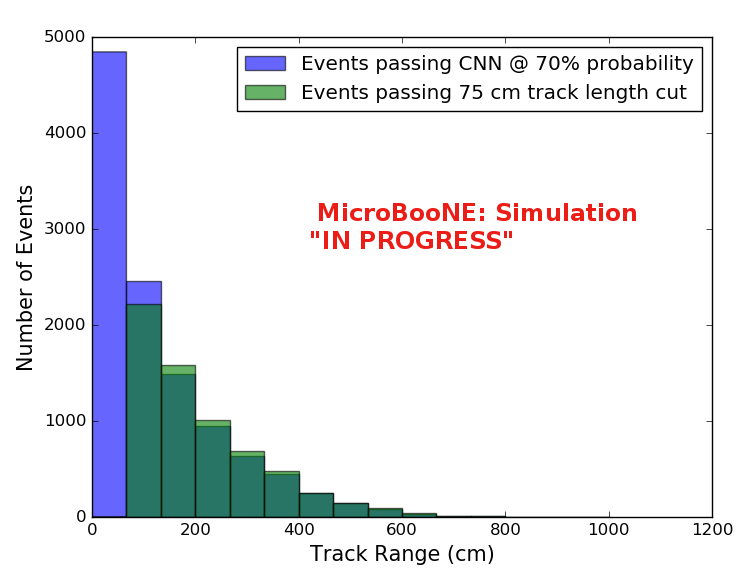
\includegraphics[width=4in,height=2.5in]{figs/sel1mod_trackrange_wrongnorm_acc70_0706.png}
	\caption{Track range distribution of events from Selection I passing CNN with 70\% accuracy}
	\label{fig:sel1mod_track}
	\end{subfigure}
	\quad
	\begin{subfigure}[b]{.45\textwidth}
	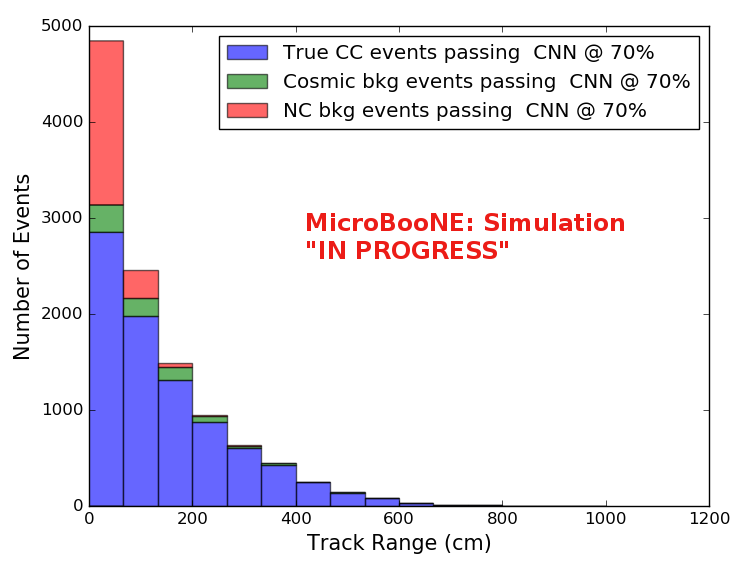
\includegraphics[width=\textwidth, height=2in]{figs/sel1mod_cnn_stackedevent_0707.png}
	\caption{Stacked signal and background track range distributions from Selection I passing CNN with 70\% accuracy}
	\label{fig:sel1mod_stackedcnn}
	\end{subfigure}
	\quad
	\begin{subfigure}[b]{.45\textwidth}
	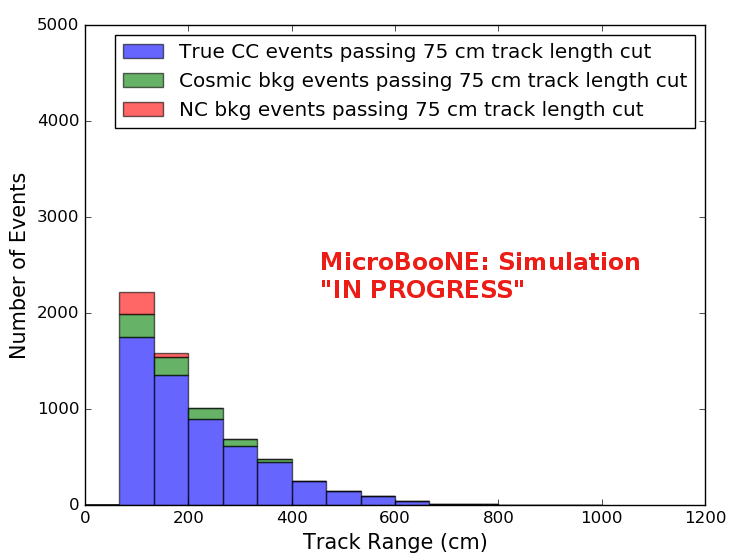
\includegraphics[width=\textwidth, height=2in]{figs/sel1mod_original_stackedevents_0707.png}
	\caption{Stacked signal and background track range distributions from Selection I passing 75 cm track length cut}
	\label{fig:sel1mod_stackedoriginal}
	\end{subfigure}
	\quad
	\begin{subfigure}[b]{.45\textwidth}
	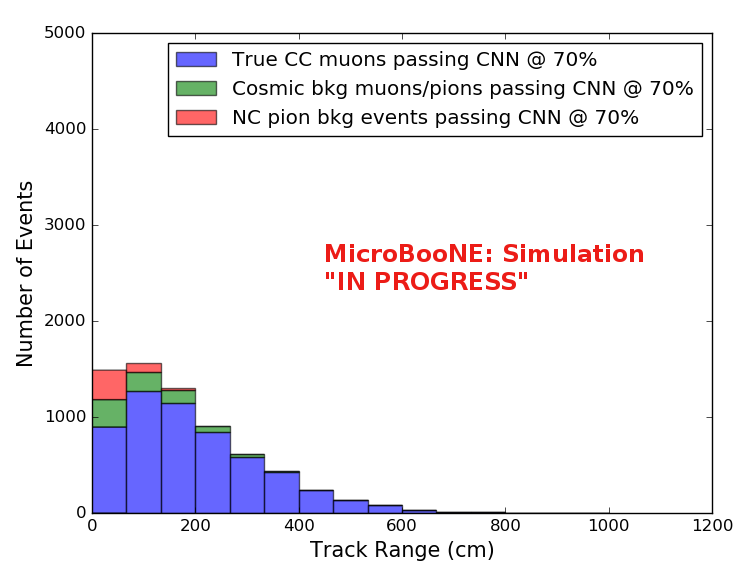
\includegraphics[width=\textwidth, height=2in]{figs/sel1mod_cnn_trackrange_mupi_acc70_0707.png}
	\caption{Stacked signal muons and background muons/pions of track range distributions from Selection I passing CNN with 70\% accuracy}
	\label{fig:sel1mod_mupi_70stackedcnn}
	\end{subfigure}
	\quad
	\begin{subfigure}[b]{.45\textwidth}
	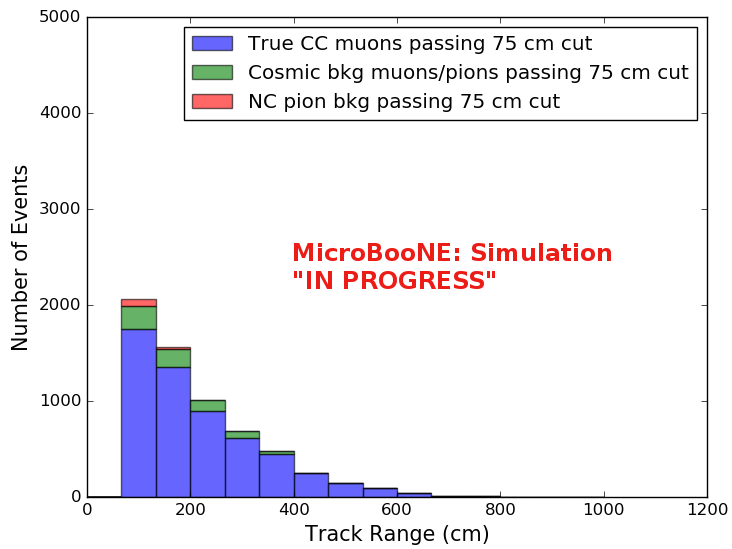
\includegraphics[width=\textwidth, height=2in]{figs/sel1mod_original_trackrange_mupi_acc70_0707.png}
	\caption{Stacked signal muons and background muons/pions of track range distributions from Selection I passing 75 cm track length cut}
	\label{fig:sel1mod_mupi_70stackedoriginal}
	\end{subfigure}
	\quad
\caption{CNN10000 distributions of track candidate images output from Selection I cc-inclusive filter}
\label{fig:sel1mod_CNN_dist}
\end{figure}



\begin{figure}[htp!]
\centering
	\begin{subfigure}[b]{.45\textwidth}
	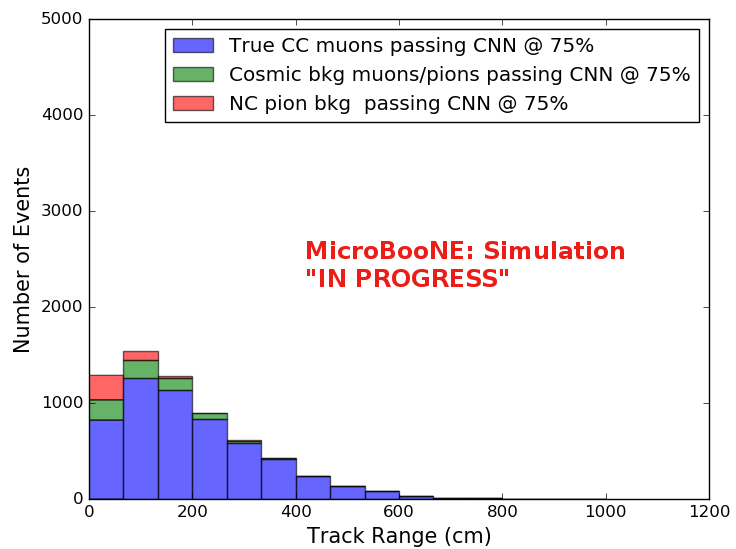
\includegraphics[width=\textwidth, height=2.5in]{figs/sel1mod_cnn_trackrange_acc75_0707.png}
	\caption{Stacked signal muons and background muons/pions of track range distributions from Selection I passing CNN with 75\% accuracy}
	\label{fig:sel1mod_mupi_75stackedcnn}
	\end{subfigure}
	\quad
	\begin{subfigure}[b]{.45\textwidth}
	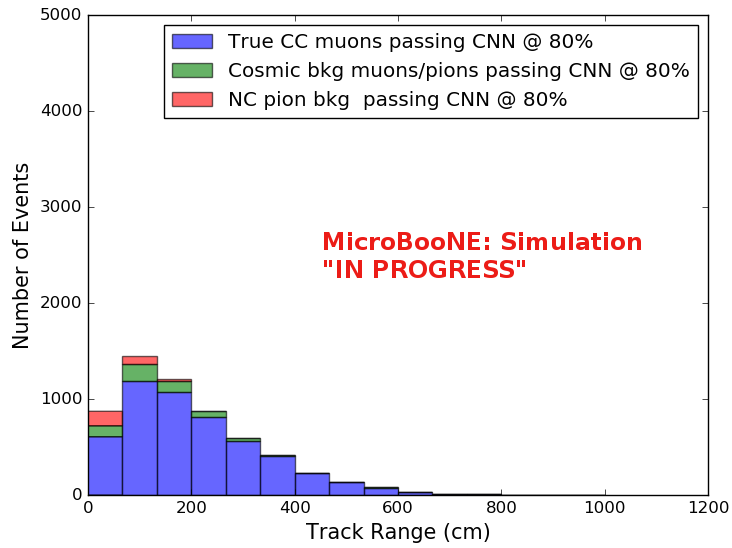
\includegraphics[width=\textwidth, height=2.5in]{figs/sel1mod_cnn_trackrange_acc80_0707.png}
	\caption{Stacked signal muons and background muons/pions of track range distributions from Selection I passing CNN with 80\% accuracy}
	\label{fig:sel1mod_mupi_80stackedcnn}
	\end{subfigure}
	\quad
	\begin{subfigure}[b]{.45\textwidth}
	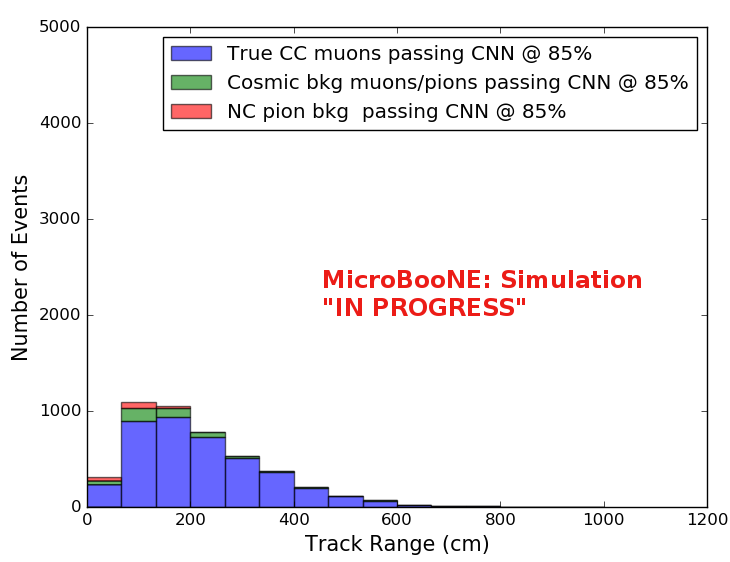
\includegraphics[width=\textwidth, height=2.5in]{figs/sel1mod_cnn_trackrange_acc85_0707.png}
	\caption{Stacked signal muons and background muons/pions of track range distributions from Selection I passing CNN with 85\% accuracy}
	\label{fig:sel1mod_mupi_85stackedcnn}
	\end{subfigure}
	\quad
	\begin{subfigure}[b]{.45\textwidth}
	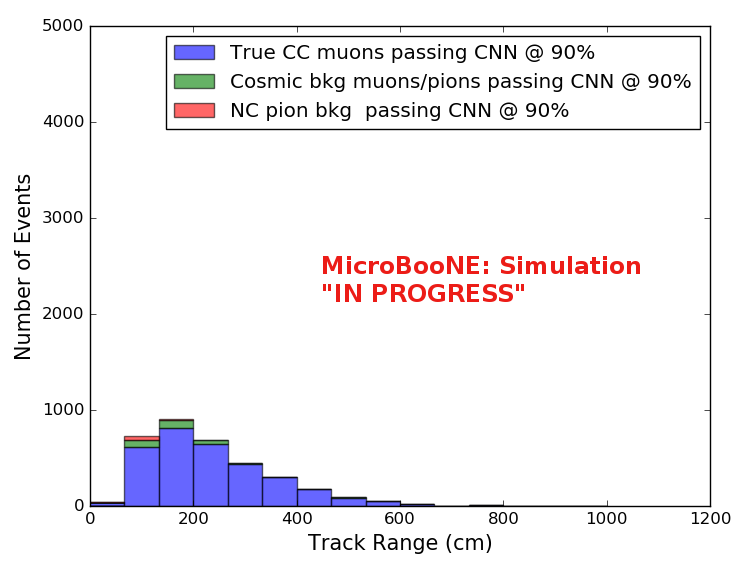
\includegraphics[width=\textwidth, height=2.5in]{figs/sel1mod_cnn_trackrange_acc90_0707.png}
	\caption{Stacked signal muons and background muons/pions of track range distributions from Selection I passing CNN with 90\% accuracy}
	\label{fig:sel1mod_mupi_90stackedcnn}
	\end{subfigure}
	\quad
\caption{CNN10000 stacked signal/background track range distributions of track candidate images output from Selection I cc-inclusive filter}
\label{fig:sel1modCNNdistacc}
\end{figure}


\begin{figure}[htp!]
\centering
	\begin{subfigure}[t]{.9\textwidth}
	\centering
	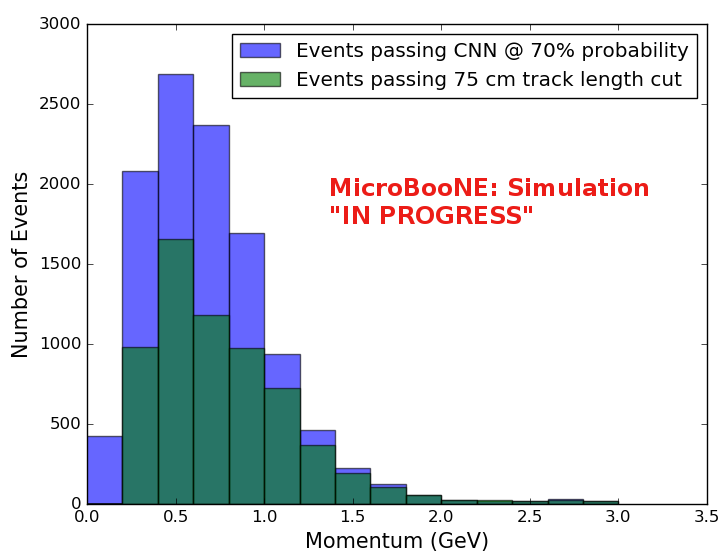
\includegraphics[width=\textwidth,height=3.5in]{figs/sel1mod_parP_wrongnorm_acc70_0706.png}
	\caption{Momentum distribution of events from Selection I passing CNN with 70\% accuracy}
	\label{fig:sel1mod_momentum}
	\end{subfigure}
	\quad
	\begin{subfigure}[t]{.45\textwidth}
	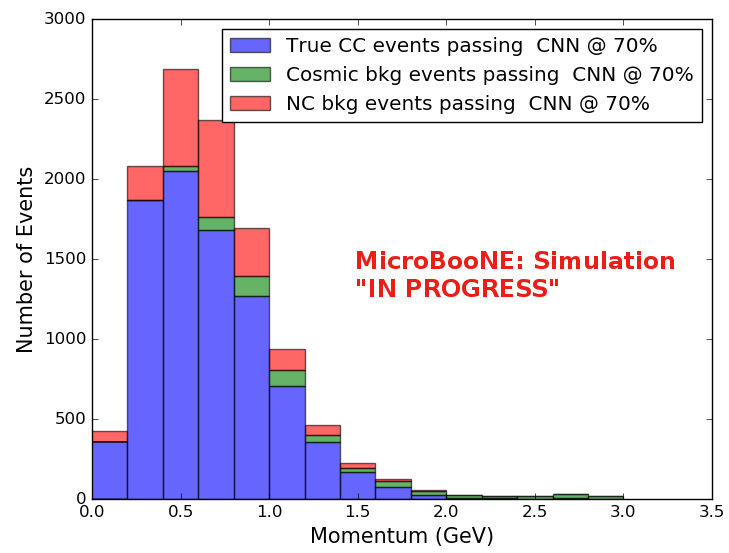
\includegraphics[width=\textwidth,height=2.5in]{figs/sel1mod_cnn_parP_stackedevents_0707.png}
	\caption{Stacked signal and background momentum distributions from Selection I passing CNN with 70\% accuracy}
	\label{fig:sel1mod_momentum_stackedcnn}
	\end{subfigure}
	\quad
	\begin{subfigure}[t]{.45\textwidth}
	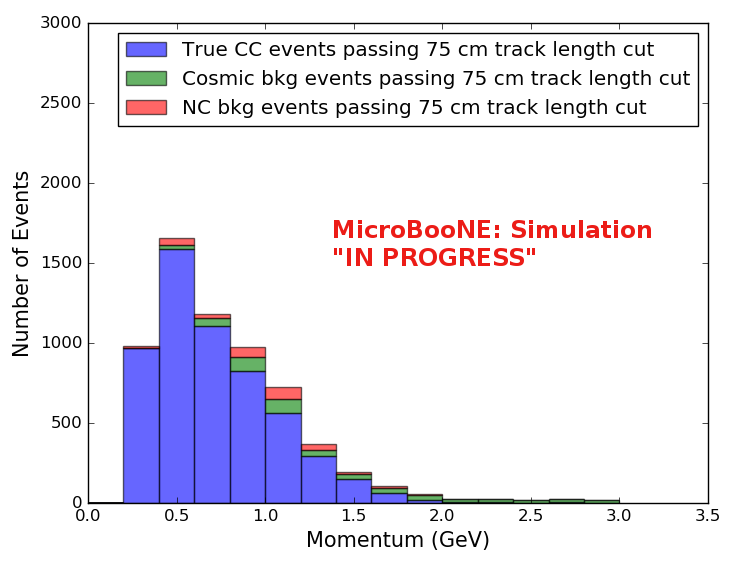
\includegraphics[width=\textwidth,height=2.5in]{figs/sel1mod_original_parP_stackedevents_0707.png}
	\caption{Stacked signal and background momentum distributions from Selection I passing 75 cm track length cut}
	\label{fig:sel1mod_momentum_stackedoriginal}
	\end{subfigure}
	\quad
\caption{CNN10000 momentum distributions of track candidate images output from Selection I cc-inclusive filter}
\label{fig:sel1mod_parP}
\end{figure}

Another check was to see if any true CC pions were passing through the cut right before the 75 cm track length cut. Figure \ref{fig:mupi} shows the comparison of the stacked track range distribution with only true CC muon signal versus the stacked distribution with true CC muons and pions signal. As you can see, we gain more events when plotting CC events with a particle type of either muons or pions due to the CNN classifying all pions in this dataset as muons. This is an interesting scenario and a sample of topologies of these images are represented in figure \ref{fig:evd}, at least 3 tracks are coming out of the vertex for these types of events. With the 75 cm track length cut, the selection is cutting event topologies like this where the pion is the tagged track candidate. Figure \ref{fig:longer_muon_badreco} has a defined longer muon track, but because of dead wires through the track, the reconstructed range is 1. less than 75 cm and 2. shorter than the reconstructed pion whose length is also less than 75 cm. This is a very interesting event, but because of issues with the tracking algorithm, the 75 cm cut would get rid of this event. The CNN was able to recover this event only because it has classified all pions as muons. Figure \ref{fig:longer_pion} shows the second case to think about, the pion, while still less than 75 cm has a reconstructed track length longer than the muon. Again, the CNN recovered this event due to pions being classified as muons. Lastly, figure \ref{fig:verylongpion} shows a pion with a reconstructed track length greater than 75 cm and the muon. These three cases show that a broader question must be asked when training the network other than is it a muon or pion. There are different routes to recover interesting events like these. One route is to ask the network ``Is it a CC event or is it an NC event?'' and obtain an image dataset consisting of whole CC/NC events that will train the network to answer this question. The other route is to ask the network ``Is this a $\mu/\pi/p/$ from a CC event or NC event and obtain an image dataset consisting of primary particles from a CC/NC event. Both these paths will be explored in future work.     

\begin{figure}[htp!]
\centering
	\begin{subfigure}[b]{.45\textwidth}
	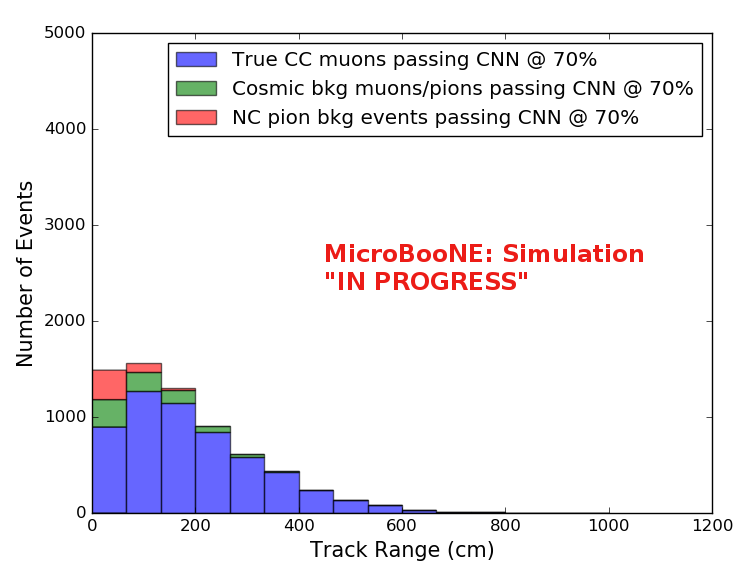
\includegraphics[width=\textwidth,height=2.5in]{figs/sel1mod_cnn_trackrange_mupi_acc70_0707.png}
	\caption{Stacked signal $\mu$/backround $\mu$ and $\pi$ track range distribution of CNN @ 70\%}
	\end{subfigure}
	\quad
	\begin{subfigure}[b]{.45\textwidth}
	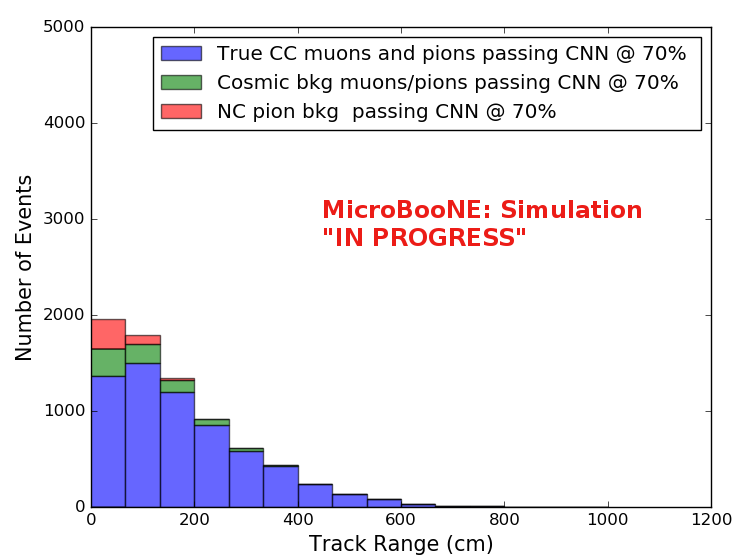
\includegraphics[width=\textwidth,height=2.5in]{figs/sel1mod_mupi_trackrange_acc70.png}
	\caption{Stacked signal $\mu \& \pi$/backround $\mu \& \pi$ track range distribution of CNN @ 70\%}
	\end{subfigure}
	\quad
\caption{Track distribution comparisons of true CC muons plotted vs true CC muons and pions plotted}
\label{fig:mupi}
\end{figure}


\begin{figure}[htp!]
\centering
	\begin{subfigure}[b]{.3\textwidth}
	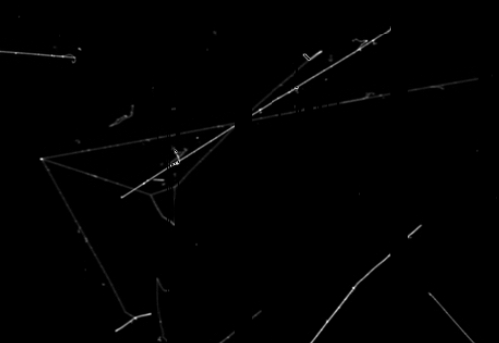
\includegraphics[width=\textwidth,height=2.5in]{figs/interesting_event.png}
	\caption{Pion recontructed track range is less than 75 cm and longer than muon track due to dead wires}
	\label{fig:longer_muon_badreco}
	\end{subfigure}
	\quad
	\begin{subfigure}[b]{.3\textwidth}
	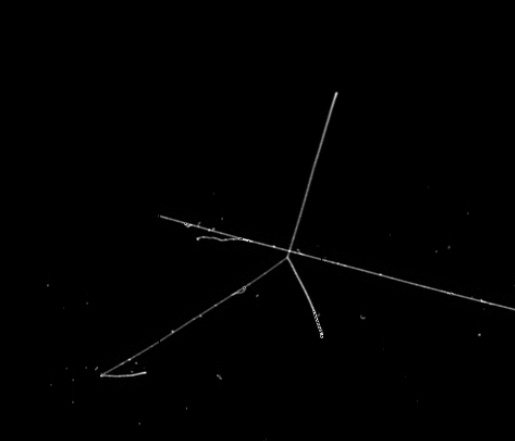
\includegraphics[width=\textwidth,height=2.5in]{figs/event2.png}
	\caption{Pion recontructed track range is less than 75 cm and larger than muon reconstructed track}
	\label{fig:longer_pion}
	\end{subfigure}
	\quad
	\begin{subfigure}[b]{.3\textwidth}
	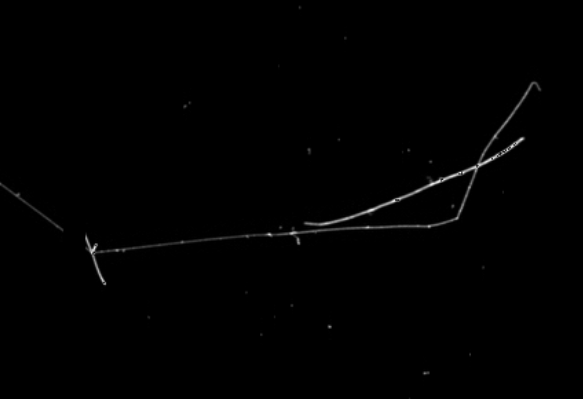
\includegraphics[width=\textwidth,height=2.5in]{figs/mupievent.png}
	\caption{Pion reconstructed track range is greater than 75 cm and larger than muon reconstructed track}
	\label{fig:verylongpion}
	\end{subfigure}
	\quad
\caption{Images of true CC events where the pion was the tagged track candidate}
\label{fig:evd}
\end{figure}

\begin{table}[htp!]
\centering
\resizebox{\textwidth}{!}{ \begin{tabular}{c||c| c c| c| c} % centered columns (4 columns)
\hline %inserts double horizontal lines
\toprule 
      && \multicolumn{2}{c}{BNB + Cosmics} & \multicolumn{1}{c}{Cosmic Only} & \multicolumn{1}{c}{Signal:}\\

      && Selection & MC Truth & &Cosmic Only \\

\midrule
75 cm Cut passing rates	& Generated Events  	       & 191362             & 45723               & 4804                & 1:22 \\ % inserting body of the table
                        & Track Containment 	       & 19391 (48\%/10\%)  & 11693 (45\%/26\%)   & 129 (38\%/2.7\%)    & 1:2.3  \\
\rowcolor{LightCyan}    & track $\geq$ 75 cm 	       & 6920 (36\%/3.6\%)  & 5780 (49\%/13\%)    & 17 (13\%/0.4\%)     & 1:0.6  \\
\hline\hline
CNN passing rates       & Generated Events  	       & 188880             & 44689               & 14606               & 1:21 \\ % inserting body of the table
		        & Track Containment 	       & 19112 ( /10\%)     & 11554 ( /26\%)      & 302 ( /2.1\%)       & 1:1.73  \\
\rowcolor{LightCyan}    & CNN cut @ 70\% Probability   & 16502 (86\%/8.7\%) & 10605 (92\%/23\%)   & 205 (68\%/14\%)     & 1:1.28  \\
\rowcolor{LightCyan}    & CNN cut @ 83\% Probability   & 7511 (46\%/4.0\%)  & 6142  (58\%/14\%)   & 32 (16\%/0.2\%)     & 1:0.4  \\
\bottomrule
\hline %inserts single line
\end{tabular}}
\caption{Comparing passing rates of CNN at different probabilities versus 75 cm track length cut: Numbers are absolute event counts and Cosmic background is not scaled appropriately. The BNB+Cosmic sample contains all events. The numbers in brackets give the passing rate wrt the step before (first percentage) and wrt the generated events (second percentage). In the BNB+Cosmic MC Truth column shows how many true $\nu_{\mu}$ CC-inclusive events (in FV) are left in the sample. This number includes possible mis-identifications where a cosmic track is picked by the selection instead of the neutrino interaction in the same event.The CNN MC True generated events were scaled wrt the MC True generated events for the 75 cm cut passing rates due to only running over 188,880 generated events versus the 191362 generated events. The last column Signal:Cosmic only gives an estimate of the $\nu_{\mu}$ CC events wrt the cosmic only background at each step. For this number, the cosmic background has been scaled as described in \cite{cc-inclusive}. Note that these numbers are not a purity, since other backgrounds can’t be determined at this step.} 
% title of Table
\label{table:passingrates} % is used to refer this table in the text
\end{table}


\begin{table}[htp!]
\centering
\resizebox{\textwidth}{!}{ \begin{tabular}{c c c|a} % centered columns (4 columns)
%\hline %inserts double horizontal lines
      &&\#Events(Fraction)  & \#Events(Fraction) \\
      &&passing Sel I & passing CNN @ 83\% Probability\\


Signal	       & $\nu_{\mu}$ CC events with true vertex in FV      & 1168(53.8\%)       & 6142(61\%)\\ % inserting body of the table
\hline\hline %inserts double horizontal lines
Backgrounds    & Cosmics Only Events                               & 725(33.4\%)       & 2582(26\%)\\ % inserting body of the table
               & Cosmics in BNB Events                             & 144(6.6\%)       & 492(4.9\%)\\ % inserting body of the table
               & NC Events                                         & 75(3.5\%)        & 778(7.7\%)\\ % inserting body of the table
               & $\nu_e$ and $\bar{\nu}_e$ Events                  & 4(0.2\%)        & 32(0.3\%)\\ % inserting body of the table
               & $\bar{\nu}_{\mu}$  Events                         & 40(1.8\%)         & 67(0.7\%)\\ % inserting body of the table
\end{tabular}}
\caption{Signal and background event numbers of selection I and selection I with CNN cut estimated from a BNB+Cosmic sample and Cosmic only sample normalized to $5*10^{19}$ PoT. The last column gives the fraction of this signal or background type to the total selected events per CNN probability.} 
\label{table:purity} % is used to refer this table in the text
\end{table}

Table \ref{table:passingrates} shows the passing rates for the 75 cm track length cut and the CNN cut at 70\% and 83\%. The passing rates at the track containment level for the 75 cm track length cut compared to the CNN are comparable with only a 0.6\% difference in the in time cosmic bin which may be due in part to the larger in time cosmic statistics used for the CNN dataset. These passing rates need to be comparable to then be able to compare the passing rates after the CNN cut to the 75 cm cut. Again, the same BNB+Cosmic sample was used for both selection I with 75 cm cut and selection I with CNN cut. As it stands, a CNN cut at 83\% probability has a MC true CC event passing rate of 14\% compared to the 13\% passing rate of the 75 cm track length cut. The Signal:Cosmic Only background is also reduced from 1:0.6 to 1:0.4 The total passing rate is also higher than the 75 cm cut, 3.6\% vs 4.0\%. Table \ref{table:purity} shows the breakdown of signal and backgrounds for the CNN at the different probabilities. We have a 61\% signal passing rate with the CNN cut @ 83\% versus the 53.8\% signal passing rate of the 75 cm cut. 

Based on these numbers, the following performance values of the selection with 75 cm cut versus selection with CNN @ 83\% probability cut were calculated:
\begin{itemize}
\item Efficiency: Number of selected true $\nu_{\mu}$ CC events divided by the number of expected true $\nu_{\mu}$ CC events with interaction in the FV.
\begin{itemize}
\item Selection I: 12.3\% 
\item Selection I with CNN10000 cut @ 83\% probability: 14\% 
\end{itemize}
\item Purity: Number of selected true $\nu_{\mu}$ CC events divided by sum of itself and the number of all backgrounds.
\begin{itemize}
\item Selection I: 53.8\% 
\item Selection I with CNN10000 cut @ 83\% probability: 61\% 
\end{itemize}
\end{itemize}

Lastly, figure \ref{fig:sel1mod_cnnperformance} shows a more representative performance of the CNN. Due to the fact that the CNN was trained on muons and pions, showing the performance of CC muon events versus NC pion events with respect to CNN probability gives a better picture of how the network is performing. Figure \ref{fig:sel1mod_cnnperformance} shows that at 83\% we are below the 75 cm cut NC pion threshold and still above the CC muon threshold. Using 83\% probability not only reduced the NC pion background, it also dramatically reduced the in time cosmics and cosmics in the BNB. 

\begin{figure}[htp!]
\centering
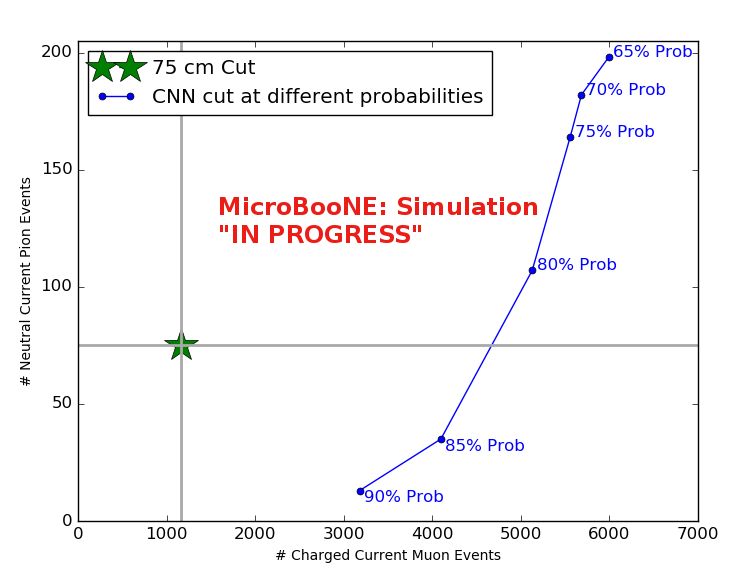
\includegraphics[width=3in,height=2.5in]{figs/cnn_performance.png}
\caption{CNN performance of classified muons and pions compared to the already implemented 75 cm track length cut}
\label{fig:sel1mod_cnnperformance}
\end{figure}

\subsection{Conclusions of CNN10000 classification of MC data}

It was shown that even though CNN10000 was trained with single particle generated muons and pions, it performs fairly well at classifying track candidate images from BNB+Cosmic events. Events have been regained below the 75 cm track length cut and the momentum and track range distributions have similar shapes to the distributions of Selection I. Efficiencies and purities were calculated for selection I events before 75 cm track length cut  with the CNN at 83\% probability and are 14\% and 62\% respectively. Although the CNN doesn't have separation between muons and pions and although all particles passing CNN are classified as muon, increasing CNN probability allows us to increase the purity as well as maintain an efficiency comparable to the 75 cm track length cut all while recovering events below that 75 cm cut. Out of the 6142 events that passed the CNN @ 83\% 1470 events were below the 75 cm cut, a recovery of 3.3\% of data with an purity of 15\%. Although these numbers are low, it is an improvement from the selecion I in both total efficiency and purity and an increase in phase space by recovering these events. 

\section{Classification using CNN100000}
For classification of BNB+Cosmics and data using CNN100000, images were made from track candidates that passed the Selection I filter, however, unlike for classifying BNB+Cosmics using CNN10000, the classification of CNN100000 went further up Selection I's cut chain. For CNN100000, steps 5 through 8 seen in section \ref{section:eventselection} were removed. The image making algorithm would then create multiple images per event of pixels corresponding to each track associated to the flattest vertex candidate in the fiducial volume. One of the findings of CNN10000 was the possibility of recovering interesting events in which a pion from a cc-inclusive event is tagged as the track candidate of interest. This was the reason for trying to expand on what a convolutional neural network could accomplish. By allowing the CNN to particle ID all track associated with the vertex candidate, we allow the selection to contain the interesting events that were cut out in selection I due to the cc pion track being chosen as the track candidate. Figure \ref{fig:cnn100000_image} shows the image making algorithm for BNB+Cosmic images. The results of using CNN100000 to classify BNB+Cosmics will be discussed in the next sections. 

\begin{figure}[htp!]
\centering
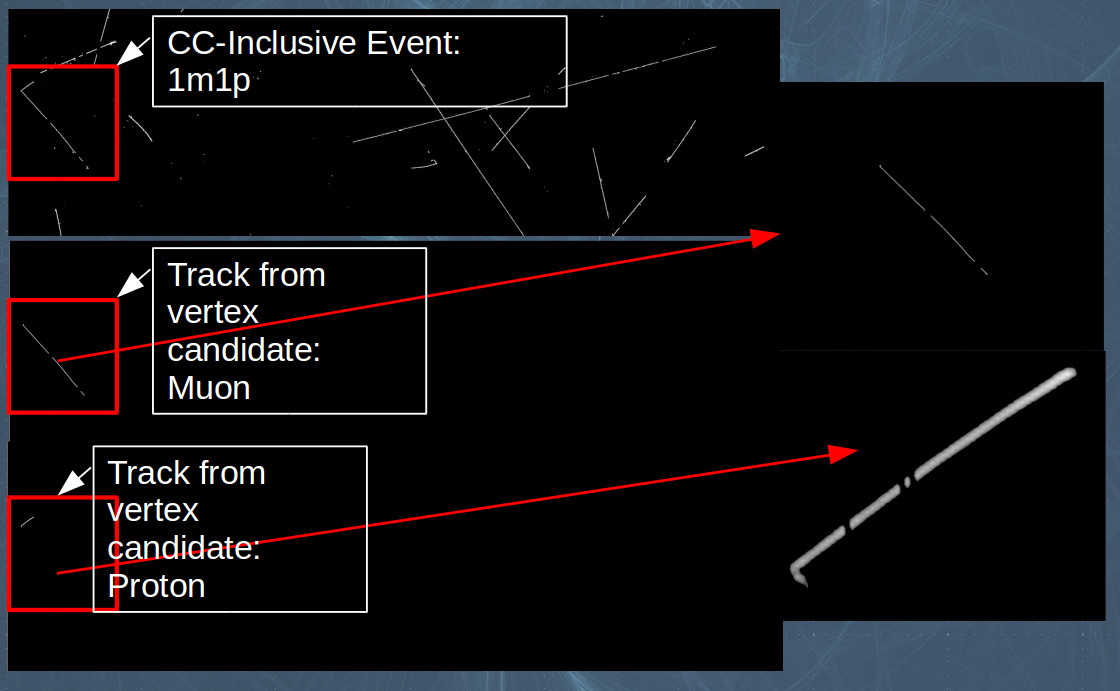
\includegraphics[width=.9\textwidth]{figs/cnn100000_image.png}
\caption{Image making steps used for classifying BNB+Cosmic events using CNN100000} 
\label{fig:cnn100000_image}
\end{figure}

\subsection{Classification of MC data using Selection I CC-Inclusive Filter}
After classifying all BNB+Cosmic and in time cosmic events, an efficiency vs purity curve was created for various muon probabilites to choose a probability that would increase both efficieny and purity of Selection I. This is shown in figure \ref{fig:roc}. Selection I and Selection II are also shown on this curve. At 85\% probability, both the efficiency and purity is better than both Selection I and Selection II therefore is the chosen muon probability. 

\begin{figure}[htp!]
\centering
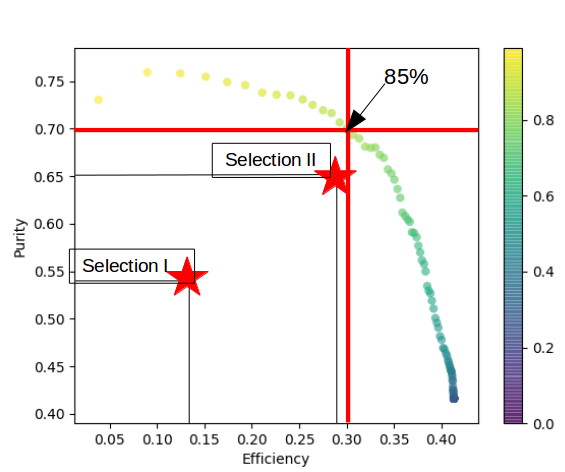
\includegraphics[width=.5\textwidth]{figs/roc_cnn_selI&II.png}
\caption{Efficiency vs Purity curve for various CNN100000 muon probabilities. At 85\% muon probability, the efficiency is 30\% and the purity is 70\%} 
\label{fig:roc}
\end{figure}

\subsubsection{Kinematic truth distributions of BNB+Cosmic events passing Selection I+CNN10000}
To classify cc-inclusive events, all images of a certain event were id'ed using CNN100000, if one image in an event was classified as an muon, that event would then be classified as a cc-inclusive event. If after running over all images in an event and none were id'ed as a muon, that event would then be classified as background. Figure \ref{fig:truthkinematics} are the true kinematic distributions for the true cc-inclusive events that passed the CNN at 85\% muon probability as well as the cc-inclusive events that passed the selection I filter.  

\begin{figure}[htp!]
\centering
	\begin{subfigure}[b]{.475\textwidth}
	\centering
		\includegraphics[width=.9\textwidth]{../bnbcosmic_output/cnn_85_trackrangedist.png}
		\caption{Track range distribution for events passing CNN10000 $\geq 85\%$ and the Selection I filter.} 
		\label{fig:cnn85trackrange}
	\end{subfigure}
	\quad
	\begin{subfigure}[b]{.475\textwidth}
	\centering
		\includegraphics[width=.9\textwidth]{../bnbcosmic_output/cnn_85_truecosthetadist.png}
		\caption{$Cos(\theta)$ distribution for events passing CNN100000 $\geq 85\%$ and the Selection I filter.} 
		\label{fig:cnn85costheta}
	\end{subfigure}
	\quad
	\begin{subfigure}[b]{.475\textwidth}
	\centering
		\includegraphics[width=.9\textwidth]{../bnbcosmic_output/cnn_85_truephidist.png}
		\caption{$\phi$ distribution for events passing CNN100000 $\geq 85\%$ and the Selection I filter.} 
		\label{fig:cnn85phi}
	\end{subfigure}
	\quad
	\begin{subfigure}[b]{.475\textwidth}
	\centering
		\includegraphics[width=.9\textwidth]{../bnbcosmic_output/cnn_85_momentumdist.png}
		\caption{Momentum distribution for events passing CNN100000 $\geq 85 \%$ and the Selection I filter.} 
		\label{fig:cnn85momentum}
	\end{subfigure}
\caption{Truth kinematic distributions of events passing CNN100000 and Selection I. The red corresponds to the Selection I passing events and blue to the CNN100000 passing events.}
\label{fig:truthkinematics}
\end{figure}

The shapes of the true kinematic distributions are comparable for CNN100000 and Selection I, however the CNN100000 curve has more events passing at muon probability 85\% compared to the Selection I filter. This is due to the removal of the containment cut. You can also see entries for cc-inclusive events at the lowest track range bin for CNN100000 that isn't there for the Selection I filter. Although the muon probability is high, we are still able to recover events with low track candidate track range. 


\begin{figure}[htp!]
\centering
	\begin{subfigure}[b]{.45\textwidth}
	\centering
		\includegraphics[width=.9\textwidth]{../bnbcosmic_output/cnn_85_trackstartXdist.png}
		\caption{X Vertex Position} 
		\label{fig:cnn85vertexX}
	\end{subfigure}
	\quad
	\begin{subfigure}[b]{.45\textwidth}
	\centering
		\includegraphics[width=.9\textwidth]{../bnbcosmic_output/cnn_85_trackstartYdist.png}
		\caption{Y Vertex Position} 
		\label{fig:cnn85vertexY}
	\end{subfigure}
	\quad
	\begin{subfigure}[b]{.45\textwidth}
	\centering
		\includegraphics[width=.9\textwidth]{../bnbcosmic_output/cnn_85_trackstartZdist.png}
		\caption{Z Vertex Position} 
		\label{fig:cnn85vertexZ}
	\end{subfigure}
\caption{Vertex position for X, Y and Z of true cc-inclusive events passing CNN100000 and Selection I}
\label{fig:vertex}
\end{figure}
\begin{figure}[htp!]
\centering
\includegraphics[width=.9\textwidth]{../bnbcosmic_output/2d85costhetaphi.png}
\caption{$Cos(\theta)$ distribution at CNN10000 $\geq 85\%$} 
\label{fig:2d85costhetaphi}
\end{figure}

\begin{figure}[htp!]
\centering
\includegraphics[width=.9\textwidth]{../bnbcosmic_output/2d85trackrangecostheta.png}
\caption{$Cos(\theta)$ distribution at CNN10000 $\geq 85\%$} 
\label{fig:2d85trackrangecostheta}
\end{figure}

\begin{figure}[htp!]
\centering
\includegraphics[width=.9\textwidth]{../bnbcosmic_output/2d85trackrangephi.png}
\caption{$Cos(\theta)$ distribution at CNN10000 $\geq 85\%$} 
\label{fig:2d85trackrangephi}
\end{figure}
\subsection{Classification of MicroBooNE data using Selection I CC-Inclusive Filter}
\subsection{Comparing two CC-Inclusive Cross Section Selection Filters}
